\section{Durchführung}
\label{sec:Durchführung}

Da die in diesem Versuch untersuchten Stoffe alle eine geringe Halbwertszeit im Bereich von Sekunden bis Stunden haben, werden die Atome erst kurz vor dem Versuch erzeugt.
Dies geschieht indem sie mit Neutronen beschossen werden.

\subsection{Erzeugung von Neutronen}

Für den Versuch wird eine Neutronen Quelle benötigt.
Diese besteht aus $\ce{^{9}_{4}Be}$-Kernen welche mit $\alpha$-Teilchen beschossen werden.
Hierdurch entsteht ein $\ce{^{12}_{6}C}$ Kern sowie ein Neutron.
Die $\alpha$-Teilchen stammen dabei aus dem Zerfall von $\ce{^{226}Ra}$-Kernen.
Da der beste Effekt erziehlt wird wenn die Neutronen eine geringe Geschwindigkeit aufweisen, werden diese gebremst.
Dafür wird die Neutronen Quelle in eine Kammer aus Paraffin gesetzt.
Ein Querschnitt dieses Aufbaus ist in Abbildung \ref{fig:quer} zu sehen.
Durch mehrfache Stöße des Neutronen mit dem Paraffin bremst dieses schließlich bis zu einer Energie ab die der mittleren kinetischen Energie der Molküle in dessen Umgebung entspricht.
So haben die Neutronen eine mittlere Geschwindigkeit von $2.2\si{\frac{\kilo\meter}{\second}}$.
Diese Neutronen werden als thermische Neutronen bezeichnet.
\begin{figure}
    \centering
    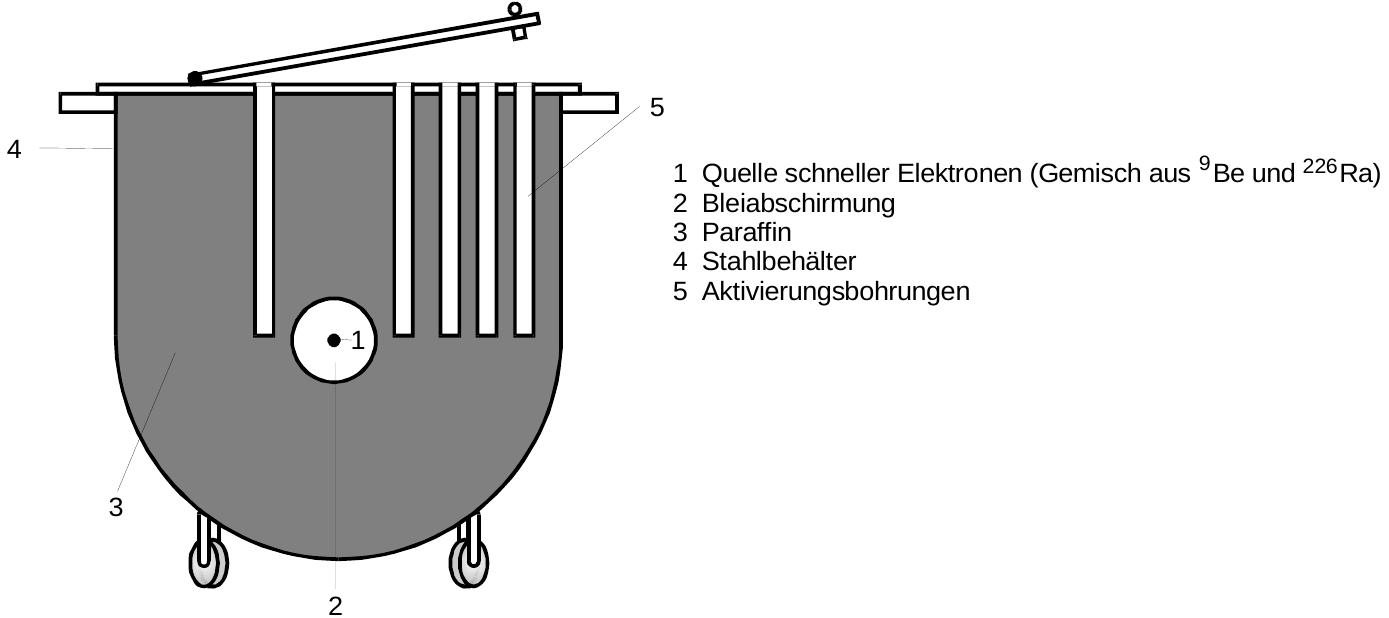
\includegraphics[width=\textwidth]{content/data/quer.png}
    \caption{Der Querschnitt des Aufbaus zur Erzeugung thermischer Neutronen. Abbildung aus Quelle \cite{anleitung} entnommen.}
    \label{fig:quer}
\end{figure}
\FloatBarrier

\subsection{Aufbau zur Messung der Halbwertszeit}

Die erzeugten Neutronen werden nun auf Atome geschossen.
Durch das zusätzliche Neutron werden diese instabil wodurch sie letztendlich zerfallen.
Der Zerfall wird durch ein Geiger-Müller-Zählrohr registriert.
Dieses gibt das Signal an einen von zwei Zählern weiter.
Die beiden Zähler wechseln periodisch.
So kann die Anzahl der Zerfälle, die der eine Zähler in einem Zeitintervall gemessen hat, einfach abgelesen werden, während der andere Zähler bereits die nächste Messung aufnimmt.
Die Probe mit dem Geiger-Müller-Zählrohr befindet sich in einer Bleiummantelung um den Effekt der natürlichen Strahlung möglichst gering zu halten.
\\\\
Um weiterhin den Nulleffekt der natürlichen Strahlung zu verringern wird zunächst eine Messung ohne Probe vorgenommen.
Dafür wird in einem Zeitintervall von $\Delta t=300\si{\second}$ die Anzahl der Zerfälle $N_\text{U}$ gemessen.
Diese Messung wird sieben mal wiederholt um eine möglichst kleine Beeinflussung zu erzielen.

\subsection{Messung zur Halbwertszeit von Vanadium}

Nachdem die Untergrundrate $N_\text{U}$ bestimmt wurde, wird mit der Messung einer Vanadium Probe begonnen.
Dafür wird die Vanadium Probe, direkt nachdem diese in der Neutronenquelle aktiviert wurde, in die Bleiummantelung gesetzt.
Das Messintervall zur Messung der Zerfälle wird hier auf $\Delta t=30\si{\second}$ gesetzt.
Die Messung wird bis zur einschließlich 42. Messung wiederholt.

\subsection{Messung zur Halbwertszeit von Rhodium}

Die Messung läuft ähnlich zur Messung von Vanadium ab.
Dieses mal wird allerdings das Messintervall auf $\Delta t = 15\si{\second}$ verringert.
Auch hier wird die Messung bis zur 42. Messung wiederholt.